\documentclass{beamer}
\usepackage{amssymb}
\usepackage{amsmath}
\usepackage[french]{babel}
\DeclareMathAlphabet{\mathmybb}{U}{bbold}{m}{n}
\newcommand{\1}{\mathmybb{1}}
\title{La formule d'Itô}

\date{\today}
\author{Lucas Lejeune, BA3-MATH-I}

\usetheme{Madrid}

\newcommand{\indep}{\perp \!\!\! \perp}
\AtBeginSection[]{
  \begin{frame}
  \vfill
  \centering
  \begin{beamercolorbox}[sep=8pt,center,shadow=true,rounded=true]{title}
    \usebeamerfont{title}\insertsectionhead\par%
  \end{beamercolorbox}
  \vfill
  \end{frame}
}
\begin{document}

\frame{\titlepage}

\begin{frame}{Table des matières}
  % \frametitle{Summary}
  \begin{enumerate}
    \item Option Call
    \item Mouvement brownien et processus stochastique
    \item Modèle de Black-Scholes
    \item Intégrale d'Itô
    \item Formule d'Itô
    \item Résolution du problème de départ
  \end{enumerate}
\end{frame}
\section{Option Call}
\begin{frame}{Option Call}{Mise en situation}
  \begin{center}
    \includegraphics[width=3cm]{imgs/police.jpg}
    \end{center}
\end{frame}
\begin{frame}{Option Call}
  \begin{block}{Definition}
    Une \textbf{option call} est un produit dérivé, contrat entre deux parties, qui donne à l'acheteur le droit (le vendeur est en revanche tenu de se plier à la décision de l'acheteur) d'acheter une quantité donnée d'un actif sous-jacent à un prix précisé à l'avance (ce prix est appelé le \textbf{strike}) (source: wikipedia.org)
  \end{block}
  \pause
  \begin{itemize}
  \item L'option n'est utilisable que le jour de sa date d'expiration
  \item On note K le \textbf{strike}.
  \item Le \textbf{payoff} est le rendement intrinsèque d'une option
    \item Une option call ne donne pas l'obligation à l'acheteur de faire valoir son option.
  \end{itemize}
\end{frame}
\begin{frame}{Option Call}
  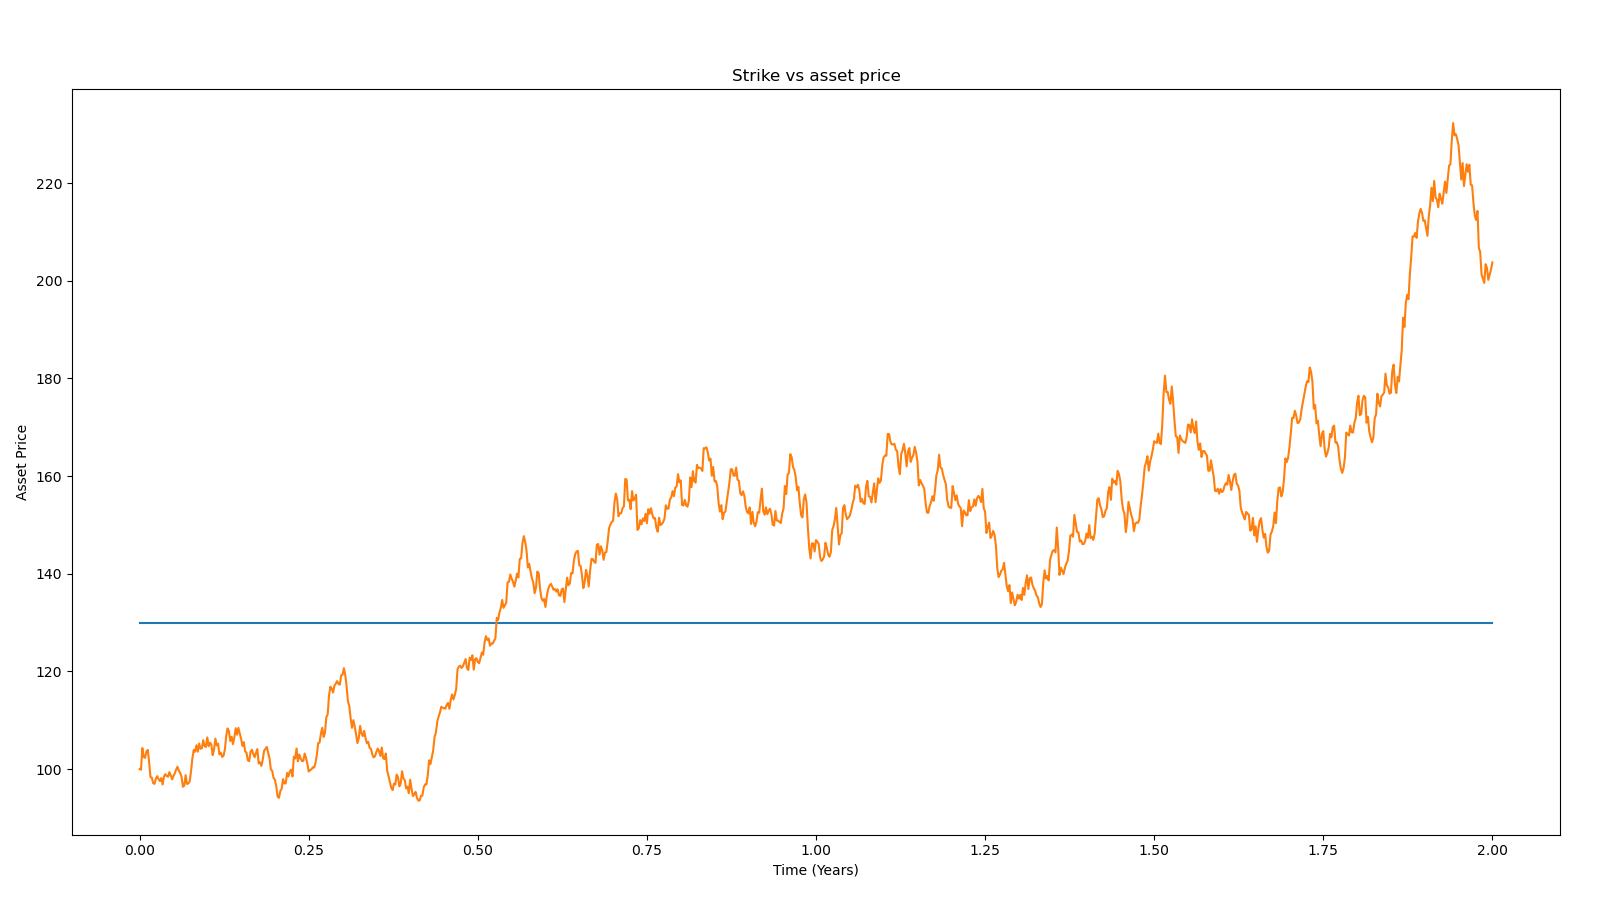
\includegraphics[width=12cm]{imgs/strike.png}
\end{frame}
\begin{frame}{Option Call}
  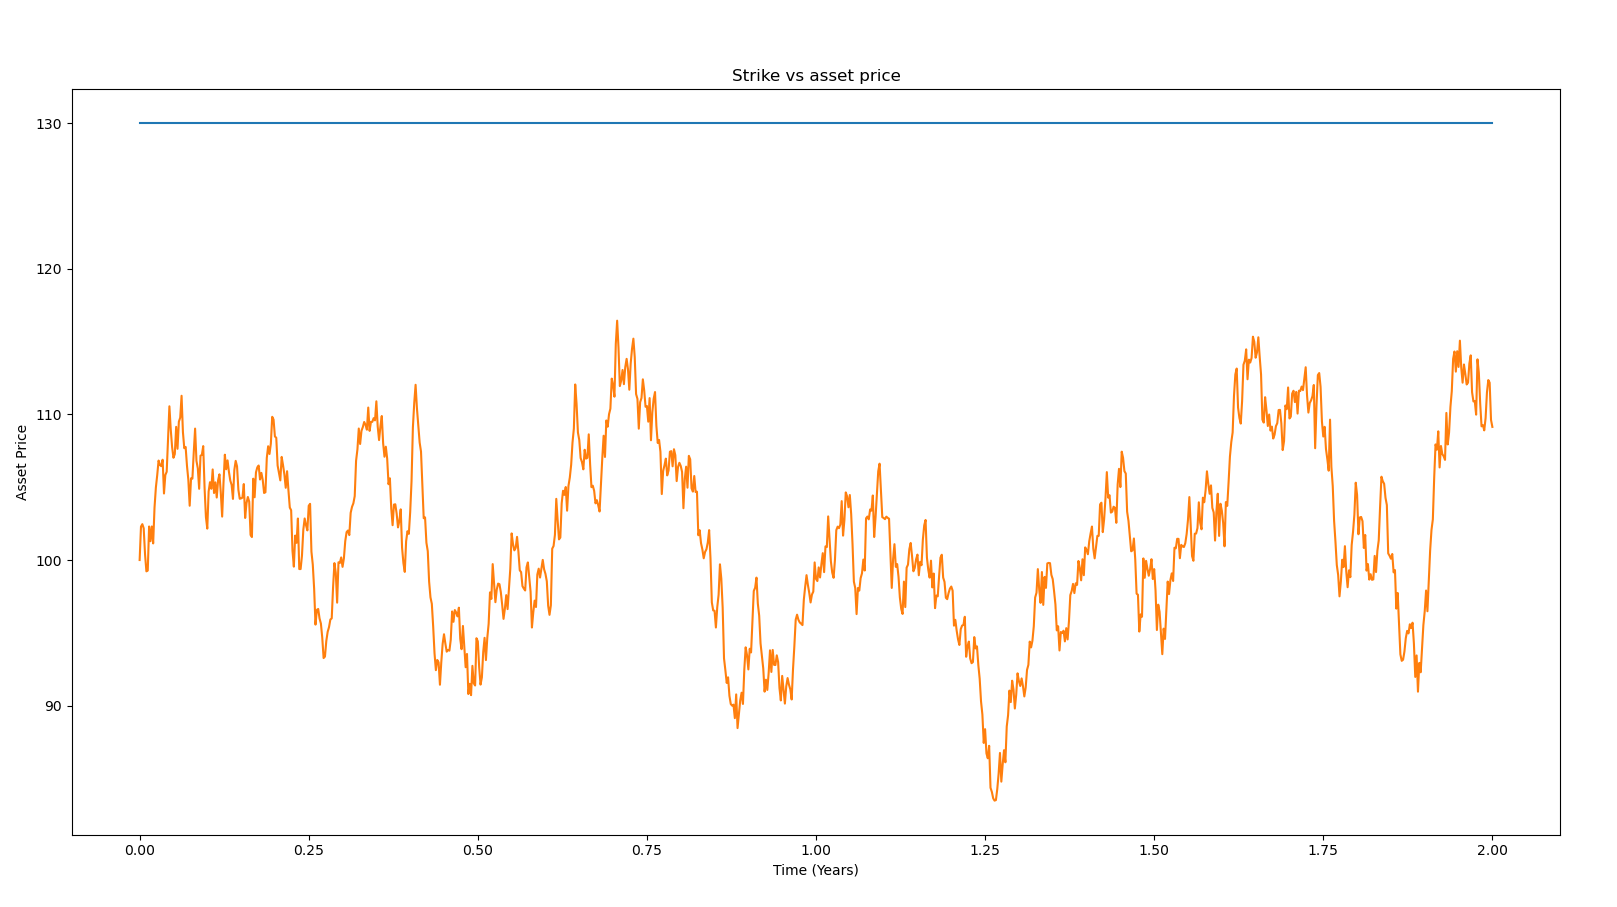
\includegraphics[width=12cm]{imgs/nostrike.png}
\end{frame}
\begin{frame}
  \begin{alertblock}{}
    \begin{center}
      Quelle serait la valeur de l'option?
      \end{center}
  \end{alertblock}
\end{frame}
\begin{frame}{Option Call}{Actualisation}
  Mettons nous dans une situation où j'achète une option effective dans 25 ans à 100€ et imaginons que l'on ne prenne pas en compte l'actualisation et donnons nous un taux d'intêrêt à 2\% par an
  \pause
  \begin{center}
    \includegraphics[width=6cm]{imgs/25ans.png}
    \end{center}
  La banque gagne donc environ 64€ sur mon achat
\end{frame}
\begin{frame}{Option Call}{Formule du pricing}
\begin{block}{Théorème fondamental du Pricing}
 Si $r$ représente le taux d'intérêt et T représente le temps, la valeur de l'obligation sera de
    \begin{equation} \label{tfp}
      \underbrace{e^{-Tr}}_{\text{fact. d'actualisation}}\mathbb{E}\left[ \text{Payoff} \right]
    \end{equation}
  \end{block}
\end{frame}
\begin{frame}{Option Call}
  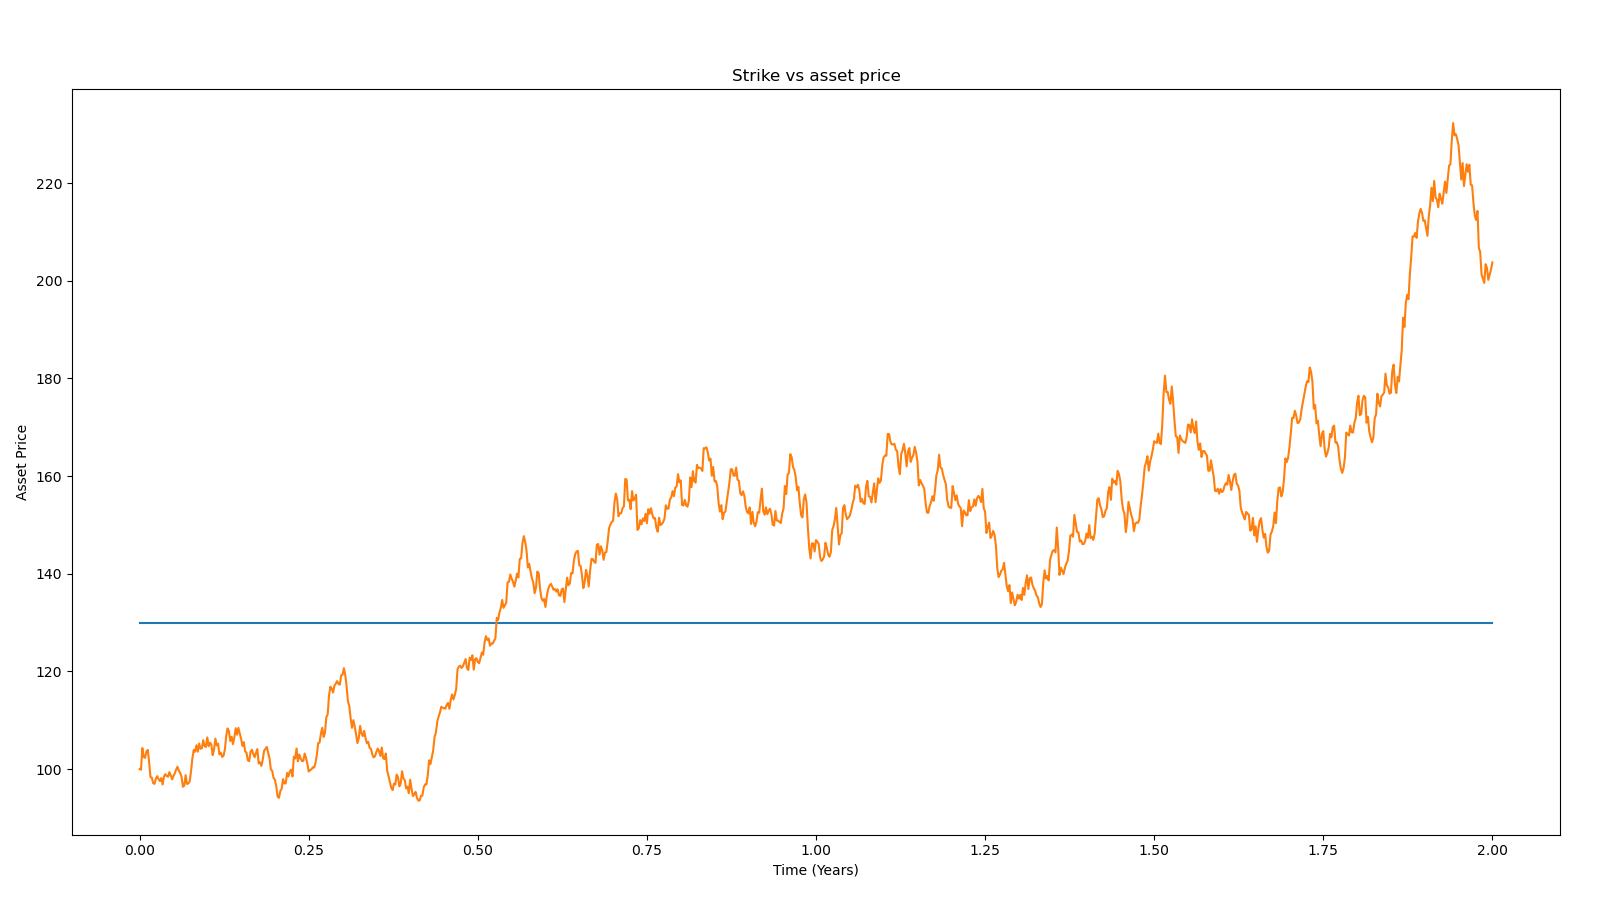
\includegraphics[width=12cm]{imgs/strike.png}
\end{frame}
\begin{frame}{Option Call}{Formule du pricing}
\begin{block}{Théorème fondamental du Pricing appliqué aux options call}
    Si $X_T$  représente le prix de l'actif sous-jacent au temps $T$, et si $r$ représente le taux d'intérêt, la valeur de l'option sera
    \begin{equation} \label{tfp}
      \underbrace{e^{-Tr}}_{\text{fact. d'actualisation}}\mathbb{E}\left[ \max \left(X_{T} - K; 0 \right) \right]
    \end{equation}
  \end{block}
\end{frame}
\section{Processus stochastiques et mouvement brownien}
\begin{frame}{Processus Stochastique}
  \begin{block}{Définition}
    Soit $T \subseteq \mathbb{R}^{+}$ et soit $\mathcal{F}$ une $\sigma$-algèbre, $\mathbb{F}$ est une \textbf{filtration} de $\mathcal{F}$ si $\mathbb{F}$ est une famille de $\sigma$-algèbres de la forme $\left( \mathcal{F}_{t}\right)_{t\in T}$ telles que
    \[
      \mathcal{F}_{s} \subseteq \mathcal{F}_{t} \subseteq \mathcal{F}, \qquad \forall s \leq t
    \]
    \end{block}
  \begin{block}{Définition}
    On appelle processus stochastique adapté la donnée
    \begin{equation}
      X = (\varOmega, \mathcal{F}, \mathbb{F}, \left(  X_{t} \right)_{t\in T}, \mathbb{P})
    \end{equation}
    où $ \varOmega $ est un ensemble, $ \mathcal{F} $ est une $\sigma$-algèbre sur $ \varOmega $, $\mathbb{P}$ est une mesure de probabilité sur $ \left( \varOmega , \mathcal{F} \right)$, $\mathbb{F}$ est une filtration et $T \subset \mathbb{R}^{+}$ représente le temps.
    Enfin, $\left( X_{t} \right)_{t\in T} $  est une famille de variables aléatoires indexées par $ T $.
  \end{block}
\end{frame}
\begin{frame}{Exemple de processus stochastique}
  \includegraphics[width=12cm]{imgs/bernoulli.png}
\end{frame}
\begin{frame}{Mouvement Brownien}
  \begin{block}{Définition}
    Un processus $ B = (\varOmega, \mathcal{F}, \left(  \mathcal{F}_{t} \right)_{t\in T},\left(  B_{t} \right)_{t\in T}, \mathbb{P} ) $ à valeurs réelles est un mouvement brownien si
    \begin{subequations}
      \begin{equation} B_{0} = 0 \qquad \mathbb{P}-p.s \end{equation}
      \begin{equation} \forall s \in \left[0, t\right], \qquad B_{t} - B_{s} \indep \mathcal{F}_{s} \end{equation}
      \begin{equation} \forall s \in \left[0, t\right], \qquad B_{t} - B_{s} \sim \mathcal{N} \left( 0, t-s\right)\end{equation}
      \end{subequations}
    \end{block}
    Le mouvement brownien est donc un type particulier de {\em marche aléatoire}.
\end{frame}
% \begin{frame}{Explication et représentation du problème}
%   \includegraphics<2>[width=7.5cm]{Kyotoimgs/overunder.png}
%   \hfill
%   \hfill \includegraphics<2>[width=7.5cm]{imgs/under.png}
% \end{frame}
\section{Modèle de Black-Scholes}
\begin{frame}{Modèle de Black-Scholes}{Mouvement Brownien Arithmétique}
  \begin{block}{Définition}
    Un processus brownien arithmétique est un processus de la forme
    \begin{equation}
      dX_{t} = \mu dt + \sigma dB_{t}
    \end{equation}
    où $\mu$ représente le drift et $\sigma$ représente la volatilitéé.
    \end{block}
  \end{frame}
  \begin{frame}{Modèle de Black-Scholes}{Influence des différents paramètres dans le mouvement brownien arithmétique}
    \includegraphics[width=12cm]{imgs/0320.png}
  \end{frame}
\begin{frame}{Modèle de Black-Scholes}
  \begin{block}{Définition}
    On va choisir de modéliser le prix d'un actif sur le marché en utilisant le processus stochastique satisfaisant l'équation stochastique suivante pour $M > 0$
    \begin{equation}
      \begin{cases}
        dX_{t} = \mu X_{t} dt + \sigma X_{t} dB_{t} \\
        X_{0} = M
      \end{cases}
      \end{equation}
      est l'équation du prix d'un actif dans le modèle de Black-Scholes. \\
    \end{block}
    \pause
    \begin{alertblock}{}
    Le but va donc être de comprendre ce processus de manière plus globale, il nous faut donc une intégrale de la forme
    \[
      X_{T} - X_{0} = \int_0^{T} \mu X_{t} dt + \int_{0}^{T} \sigma X_{t} dB_{t}
    \]
  \end{alertblock}
  \pause
  Le but va donc maintenant être de définir cette intégrale
\end{frame}
 \begin{frame}{Représentation de cinq $X_{t}$}{$\mu =0.1, \sigma =0.3$}
   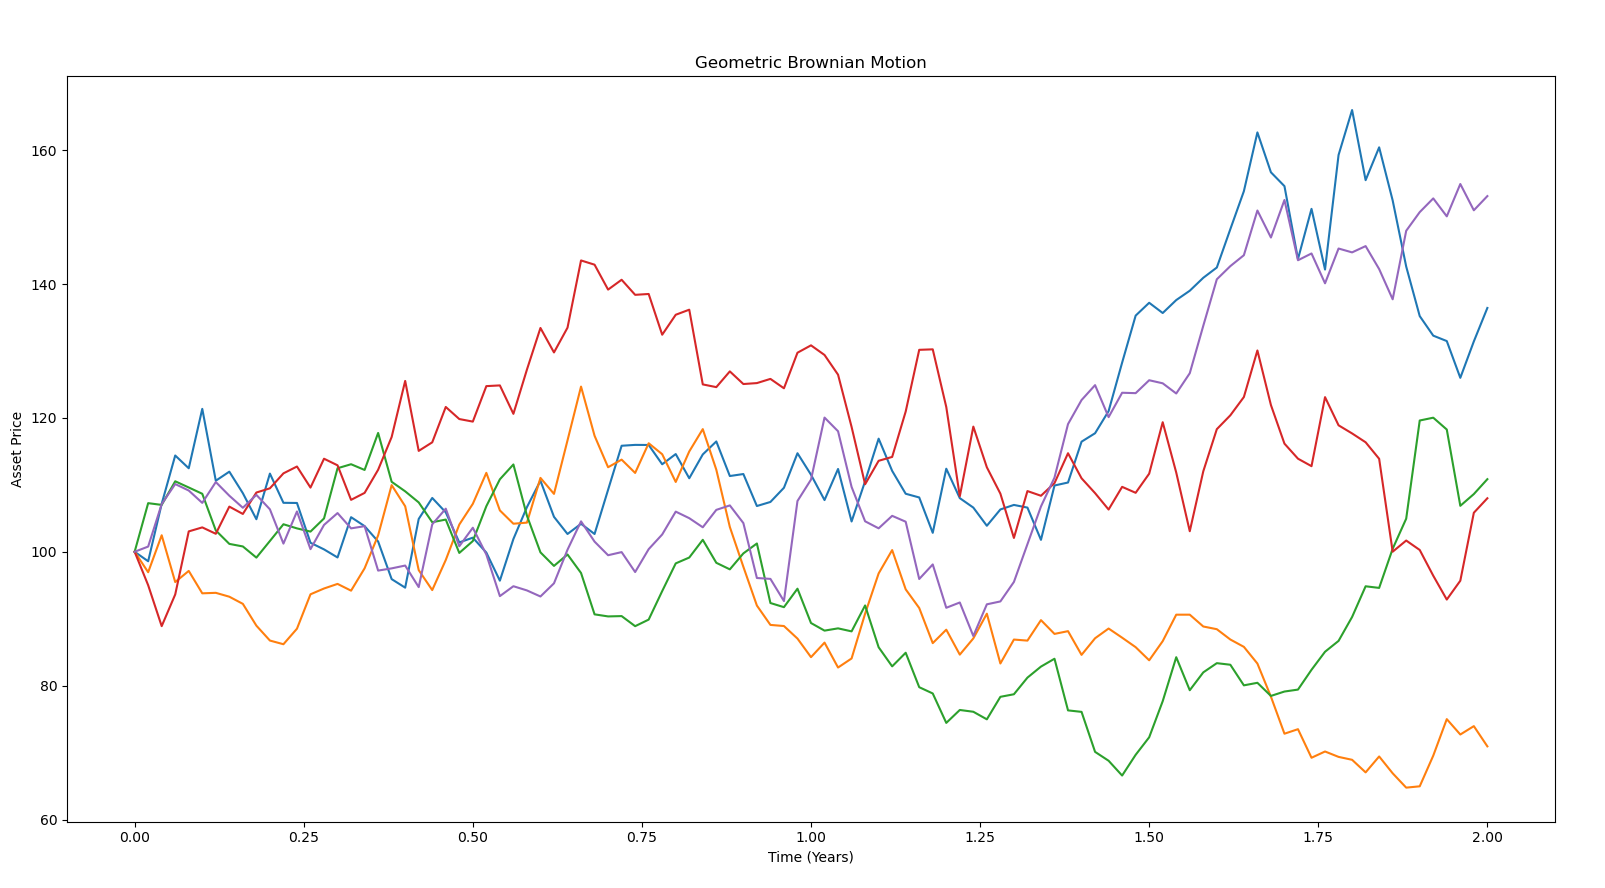
\includegraphics[width=12cm]{imgs/bs5.png}
 \end{frame}
 \begin{frame}{Représentation de cinq $X_{t}$}{$\mu =2, \sigma =0.3$}
   \includegraphics[width=12cm]{imgs/mu2.png}
 \end{frame}
 \section{Construction de l'intégrale d'Itô}
 \begin{frame}{Construction de l'intégrale d'Itô}
   \begin{block}{Définition}
     Soit $ T \in \mathbb{R}^{+}$, $\mathcal{B}$ les boréliens de $ \left[0; T  \right]$, et soit $ (\mathcal{F}_{t})_{t \geq 0}$ la filtration du mouvement brownien. On définit $\mathcal{H}^{2}_{0}$ comme l'ensemble des fonctions mesurables sur $\mathcal{B} \otimes \mathcal{F}$ telles que celles-ci soient de la forme \iffalse [[ \fi
     \[
       \forall \omega \in [0; T], \qquad f(\omega, t) = \sum_{i=0}^{n-1}a_{i}(\omega) \1_{\left] t_{i} ; t_{i+1} \right] }
     \]
     avec $a_{i} \in \mathcal{F}_{t_{i}}$, $\mathbb{E}\left[ a_{i}^{2} \right] < \infty$ et $0 = t_{1} < t_{2} < \cdots < t_{n} = T$
     \end{block}
    \end{frame}

    \begin{frame}{Construction de l'intégrale d'Itô}{Définition de l'intégrale d'Itô sur $\mathcal{H}^2_0$}<1->
      \begin{block}{Propriétés de base de l'intégrale}
        Notre intégrale devrait être définie sur $\mathcal{H}^{2}_{0}$, celle-ci devrait être un opérateur linéaire, de plus
     \iffalse [ [ \fi  si $ f(\omega, t) = \1_{\left] a; b \right]} $ on aimerait
     \[
       I(f)(\omega) = \int_{a}^{b}f(\omega, t) dB_{t} = B_{b} - B_{a}
     \]
   \end{block}
     \begin{block}{Définition}<2->
       Soit $ f \in \mathcal{H}^{2}_{0} $ on va définir l'intégrale d'Itô comme étant
       \[
         \forall \omega \in [0; T], \qquad I(f)(\omega) = \sum_{i=0}^{n-1} a_{i}(\omega)\left( B_{t_{i+1}} - B_{t_{i}} \right)
       \]
     \end{block}
   \end{frame}
   \begin{frame}{Construction de l'intégrale d'Itô}{Lemme d'Isométrie d'Itô}
     \begin{block}{Lemme d'isométrie d'Itô}
       Soit $f \in \mathcal{H}_{0}^{2}$, alors on a
       \[
         \Vert I(f) \Vert_{L^{2}(dP)} = \Vert f \Vert_{L^{2}(dP \times dt)}
       \]
     \end{block}
     \end{frame}
    \begin{frame}{Construction de l'intégrale d'Itô}{Preuve du lemme d'isométrie}
       On calcule d'abord le membre de droite de l'équation, remarquons donc que
       \iffalse [  \fi
       \[
       f ^{2}(\omega, t) = \sum_{i=0}^{n-1}a^{2}_{i} \1 _{\left( t_{i} ; t_{i+1} \right]}
     \]
     \pause
     et donc
     \[
      \Vert f \Vert _{L^{2}(dP \times dt)} =\mathbb{E} \left[ \int_{0}^{T} f^{2} (\omega, t) dt \right] = \sum_{i=0}^{n-1} \mathbb{E}\left[  a^{2}_{i}\right] (t_{i+1} - t_i)
    \]
  \end{frame}
  \begin{frame}{Suite preuve}
  On calcule maintenant le membre de gauche de cette équation
  \pause
    \[
    \begin{aligned}
      \Vert I(f) \Vert _{L^{2}(dP)} &= \mathbb{E}\left[ I(f)^{2} \right] \\ \pause
                                    &= \sum_{i=0}^{n-1} \mathbb{E} \left[a^{2}_{i} \left( B_{t_{i+1}} - B_{t_{i}} \right)^{2} \right] \\ \pause
      &= \sum_{i=0}^{n-1} \mathbb{E} \left[ a_{i}^{2} \right] (t_{i+1} - t_{i})
    \end{aligned}
  \]
  \pause
  On conclut la preuve en remarquant que $\Vert I(f) \Vert _{L^{2}(dP)} = \Vert f \Vert _{L^{2}(dP \times dt)}$.
     \end{frame}
     \begin{frame}{Construction de l'intégrale d'Itô}
   \begin{block}{Définition}<1->
     Soit $T \in \mathbb{R}^{+}_{0}$, $\mathcal{B}$ les boréliens de $\left[0; T  \right]$ et $\left( \mathcal{F}_{t} \right)_{t\in T}$ une filtration naturelle de $B_{T}$.
     On définit $\mathcal{H}^{2}$ comme étant l'espace des fonctions mesurables sur $F_{T} \otimes \mathcal{B}$, telles que pour tout $ t \in \left[0; T  \right], \omega \mapsto f(\omega, t)$ est mesurable sur $\mathcal{F}_{t}$ et respectant la condition d'intégrabilité \\
     \[
       \mathbb{E}\left[\int_{0}^{T}f^{2}(\omega, t) dt \right] < \infty
     \]
   \end{block}
   \pause
   \begin{block}{Théorème}
     $\mathcal{H}^{2}_{0}$ est dense dans $ \mathcal{H}^{2}$, et on peut donc prolonger la définition de $I$ par continuité sur tout $\mathcal{H}^{2}$.
   \end{block}
 \end{frame}
 \section{Lemme d'Itô}
   \begin{frame}{Lemme d'Itô}{Cas simple}
     \begin{block}{Lemme d'Itô}
       Avec $f: \mathbb{R} \rightarrow \mathbb{R} $ de classe $\mathcal{C}^{2} $, on a
       \begin{equation}
         f(B_{t}) = f(0) + \int_{0}^{t}f'(B_{S})dB_{S} + \frac{1}{2}\int_{0}^{t} f''(B_{s})ds
       \end{equation}
     \end{block}
     \end{frame}
     \begin{frame}{Lemme d'Itô}{Application}
       Calculons $ \int_{0}^{t} B_{s}dB_{s}$.
       \pause
       Posons
       \[
         f: x \mapsto \frac{x^{2}}{2}
       \]
       \pause
       appliquer le lemme d'Itô à f donne pour $ t \in \mathbb{R}^{+}$
       \begin{align}
         \int_{0}^{t}f'(B_{s})dB_{s} &= f(0) - f(B_{t}) + \int_{0}^{t} f''(B_{s}) ds \\
         &= - \frac{B_{t}^{2}}{2} + t
       \end{align}
       \pause
       Et donc
       \[
         \int_{0}^{t}B_{s}dB_{s} = - \frac{B_{t}^{2}}{2} + t
       \]
     \end{frame}
     \begin{frame}{Lemme d'Itô}{Plusieurs variables}
     \begin{block}{Lemme d'Itô, avec plusieurs variables}<1->
       Soit $f\in \mathcal{C}^{1, 2}(\mathbb{R}^{+} \times \mathbb{R})$, on a
       \begin{equation}
           f(t, B_{t}) = f(0, 0) + \int_{0}^{t}\frac{\partial f}{\partial x}(s, B_{s}) dB_{s} + \int_{0}^{t}\frac{\partial f}{\partial t}(s, B_{s}) ds + \frac{1}{2} \int_{0}^{t}\frac{\partial ^{2} f}{\partial x^{2}}(s, B_{s}) ds
         \end{equation}
         \end{block}
       \begin{block}{Lemme d'Itô (notation)}<2->
         Soit $f\in \mathcal{C}^{1, 2}(\mathbb{R}^{+} \times \mathbb{R})$, et $ X_{t} = f(t, B_{t})$ un processus stochastique, on écrira
         \begin{equation}
           dX_{t} = \frac{\partial f}{\partial x}(t, B_{t}) dB_{t} + \frac{\partial f}{\partial t}(t, B_{t}) dt + \frac{1}{2} \frac{\partial^{2}f}{\partial x^{2}}(t, B_{t}) dt
         \end{equation}
       \end{block}
     \end{frame}
     \section{Résolution du problème de départ}
   \begin{frame}{Résolution du problème de Black-Scholes}
     On reprend notre équation stochastique modélisant le prix des actifs
     \begin{equation}
       dX_{t} = \mu X_{t} dt + \sigma X_{t} dB_{t}
     \end{equation}
     \pause
     et on s'intéresse à $d \ln X_{t}$ en y appliquant la formule d'Itô
     \[
       d \ln X_{t} = \frac{1}{X_{t}} dX_{t} - \frac{1}{2X^{2}_{t}} dX_{t} \cdot dX_{t}
     \]
     \pause
     En développant $dX_{t}$ on trouve
     \[
       d \ln X_{t} = \frac{1}{X_{t}} \left( \mu X_{t} dt + \sigma X_{t} dB_{t} \right) - \frac{1}{2X_{t}^{2}} \left( \mu X_{t} dt + \sigma X_{t} dB_{t} \right) \left( \mu X_{t}dt + \sigma X_{t} dB_{t}\right)
     \]
     \end{frame}
    \begin{frame}{Résolution du problème de départ}{Box-Calculus}
       \begin{block}{Box-Calculus}
         \begin{center}
           \begin{tabular}{|c|c|c|}
             \hline
             $\cdot$ & $dt$ & $dB_t$ \\
             \hline
             $dt$ & 0 & 0 \\
             $dB_{t}$ & 0 & $dt$ \\
             \hline
           \end{tabular}
         \end{center}
         \end{block}
       \end{frame}
       \begin{frame}{Résolution du problème de départ}
    \[
       d \ln X_{t} = \frac{1}{X_{t}} \left( \mu X_{t} dt + \sigma X_{t} dB_{t} \right) - \frac{1}{2X_{t}^{2}} \left( \mu X_{t} dt + \sigma X_{t} dB_{t} \right) \left( \mu X_{t}dt + \sigma X_{t} dB_{t}\right)
     \]
     \pause
     En appliquant le Box-Calculus, on simplifie notre dernière expression
    \[
       d \ln X_{t} =  \mu dt + \sigma dB_{t} - \frac{\sigma^{2}}{2} dt
     \]
     \[
       d \ln X_{t} = \left( \mu - \frac{\sigma^{2}}{2} \right) dt + \sigma dB_{t}
     \]
     \pause
     On intègre ensuite de chaque côté de l'équation avec l'intégrale d'Itô
     \[
       \int_{0}^{T} d \ln \left(  X_{t} \right) = \int_{0}^{T} \left(\mu - \frac{\sigma^{2}}{2} \right) dt + \int_{0}^{T} \sigma dB_{t}
     \]
     \pause
     \[
       \ln \left(\frac{X_{T}}{X_{0}} \right) = \left( \mu - \frac{\sigma^{2}}{2} \right) T + \sigma B_{T}
     \]
        \end{frame}
   \begin{frame}{Déduction de la formule de Black-Scholes}
\begin{equation} \label{eq:9}
       X_{T} = X_{0} \exp \left(  \left( \mu - \frac{\sigma^{2}}{2} \right) T + \sigma B_{T} \right)
     \end{equation}

     \pause
     \begin{block}{Définition}
       Soit $Z \sim \mathcal{N}\left(0, 1 \right)$, et soient $\mu \in \mathbb{R}$ et $\sigma \in \mathbb{R}^{+}$, alors la variable définie par $ X = e^{\mu + \sigma Z}$ suit une loi log-normale.
     \end{block}
     On reprend donc $ \ref{eq:9} $ pour voir que $X_{T} \sim \log \mathcal{N} \left( \left( \mu - \frac{\sigma^{2}}{2} \right) T + \ln X_{0}; \sigma \sqrt{T}  \right)$ \\
     \pause
     Tout ce qu'il reste à faire est alors de calculer $\mathbb{E}\left[\max(X_{t} - K; 0)e^{-tr}\right]$ où $ X_{t}$ suit une log-normale.
   \end{frame}
   \begin{frame}{Formule de Black-Scholes}
     Nos calculs précédents nous donnent finalement la formule de Black-Scholes telle qu'étudiée en actuariat
     \begin{block}{Théorème}
       Dans le modèle de Black-Scholes, la valeur d'une option call est donné par la formule
       \begin{equation}
         X_{0}\varPhi(d_{1}) - Ke^{-rT}\varPhi(d_{2})
       \end{equation}
       où
       \[
         d_{1} = \frac{1}{\sigma \sqrt{T}} \left( \ln \left(\frac{X_{0}}{K} \right) + \left( r + \frac{\sigma^{2}}{2} \right)T \right)
       \]
       et
       \[
         d_{2} = d_{1} - \sigma \sqrt{T}
       \]
    \end{block}
  \end{frame}
  \begin{frame}{Application à la situation de départ}
    On analyse le marché, et on trouve $ \sigma = 0.3$ ainsi que $ \mu = 0$, de plus le taux d'intérêt sans risque est à $r = 0.02$ appliquer Black-Scholes nous donne finalement que l'option a une valeur de $8.91€$€
  \end{frame}
  \section{Limites du modèle}
  \begin{frame}{Limites du modèle}
    \begin{enumerate}
      \item Le modèle est trop théorique
            \pause
      \item Sous-estimation des événements extrêmes
            \pause
      \item Beaucoup de suppositions non-vérifiées empriquement afin de rendre le modèle simple
            \pause
            \item etc.
    \end{enumerate}
  \end{frame}
  \begin{frame}{Merci!}
    \includegraphics[width=12cm]{imgs/100b.png}
  \end{frame}
\end{document}
